\chapter{Cahier des charges}
\section*{Chronogramme}
\begin{center}
\end{center}
\section{Remise en contexte}
\paragraph{Les vulnérabilités de type Use-After-Free}
\subparagraph{}
La plupart des vulnérabilités enseignées et étudiées dans le cadre scolaire
se rapportent à des fonctionnement souvent statique, ou du moins dont le comportement
est uniquement lié au programme ciblé en lui-même (à son architecture de compilation et/à
son code source). On prendra comme exemple les dépassements de tampons, les problèmes de
formattage des chaines de caractères, etc.\subparagraph{}
Dans l'environnement industriel, et sur les solutions importantes utilisées dans le monde
de l'entreprise, ces vulnérabilités sont de plus en plus rare. Premièrement parce que le temps
faisant son oeuvre, la grande majorité ont été reportées sur les solutions les plus anciennes,
mais également parce que de nombreux outils pouvant les détecter rapidement (parfois dès la compilation)
ont été concus.\subparagraph{}
Les attaquants explorent donc de nouvelles voies, notamment sur des problèmatiques plus dynamiques, et/ou
lié également à l'environnement de production du programme, comme le système d'exploitation ou la bibliothèque utilisée.
En effet, de nombreuses opérations du programme dépendent intrisequement du système d'exploitation sous-jacent et
même si le comportement final reste souvent le même sur les differentes plateformes, les effets colateraux
sur le contexte et le mécanisme d'execution est souvent différent.\subparagraph{}

\subparagraph{L'évolution des vulnérabilités de type use-after-free}
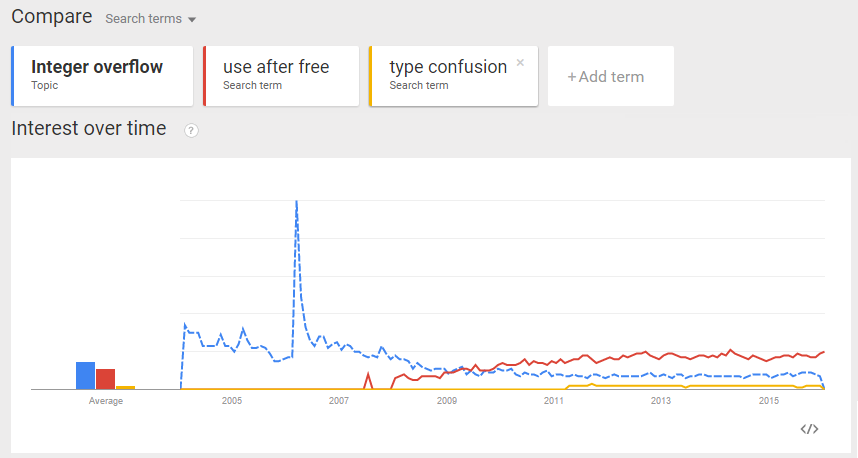
\includegraphics[scale=0.5]{histogramme-uaf.png}\newline
Beaucoup de problème de corruption mémoire sont directement dû à la mauvaise utilisation
du language utilisé pour le developpement. En effet, les languages de programmation tels que C
ou C++ demandent une gestion de la mémoire manuelle (le C++ permet néanmoins une gestion plus ou moins automatisée
avec les nouveaux standards).
\subparagraph{}
Il est donc fréquent de rencontrer des erreurs sur ce point là. Cela arrive
notamment lorsque par un problème de maintenabilité ou de mauvaise conception, la partie du programme devant
libérer une zone mémoire est méconnue/non documentée.\subparagraph{}
Ce n'est cependant pas toujours le cas et les allocateurs de mémoires / ramasse-miettes sont parfois en cause.

\subparagraph{Exemple}
Un exemple très simple et souvent rencontré dans la littérature est le suivant:
\begin {lstlisting}[frame=single]
int main(void)
{
    int *a = malloc(sizeof(int));
    *a = 5;
    free(a);
    int *b = malloc(sizeof(int));
    printf("\%d", *b); // affiche 5
    *b = 7;
    printf("\%d", *b); // affiche 7
    *a = 10;
    printf("\%d", *b); // affiche 10
}
\end{lstlisting}
\subparagraph{}
Sur une distribution Linux classique comme Ubuntu, quelque soit la taille de mots
de l'architecture (32 ou 64 bits), les adresses a et b sont exactement les mêmes.
Cela est directement dû à l'algorithme d'allocation mémoire de la bibliothèque standard
C.\subparagraph{}
En effet lors du premier appel à la fonction \textbf{malloc()}, une première zone est allouée.
Lors de sa libération, la zone libérée est mise en cache, et lors du second appel à \textbf{malloc()},
l'algorithme va retourner la même zone mémoire. Ce comportement ne sera pas détaillée dans cette section, car
il demanderait à lui seul plusieurs pages.\subparagraph{}
Cela va de soi que cet exemple est simpliste, et que les vulnérabilités rencontrées en production sont
rarement aussi visible. Il permet toutefois de bien visualiser l'origine du problème.


\paragraph{Outils existants en dynamique et en statique}
Des outils simplistes ne suffisent pas à détecter la présence d'use-after-free.\newline
Par exemple, si une solution détecte uniquement l'accès à une zone mémoire non allouée, l'exemple
donnée précedemment ne sera pas considéré comme vulnérable, car la zone mémoire est là même pour deux
allocations différentes. Plusieurs possibilités s'ouvrent alors : l'analyse statique, l'analyse dynamique,
et un mélange des deux.

\paragraph{Analyse dynamique}
De nombreuses personnes / équipes se sont penchées sur la détection de ces comportements, dynamiquement et
statiquement. Nous parlerons tout d'abord des solutions dynamiques existantes, puis nous aborderons \textbf{les approches
statiques, qui sont directement liées au sujet de ce stage.}

\subparagraph{Kasan: Kernel Address Sanitizer}
Kasan est un projet open-source, développée majoritairement
par les acteurs du noyaux Linux ainsi que par Google. Son but est d'ajouter une couche de protection
mémoire au noyau Linux afin de détecter certains corruptions mémoires dans les opérations du noyau, comme
des use-after-free ou des accès hors limites.
https://github.com/google/kasan

\subparagraph{AddressSanitizer}
AddressSanitizer est également un projet open-source, et effectue
un travail similaire à Kernel Adress Sanitizer. Intégré dans la base de code de
LLVM, il permet, lorsque le programme testé est compilé avec les bonnes options du compilateur \textbf{Clang},
de détecter des problèmes de mémoires.

\subparagraph{Undangle}
Undangle est également un exemple connu, spécialement dédié à la découverte de vulnérabilité
de type use-after-free et double-free, à partir d'une trace d'execution. Il a été développé par plusieurs
personnes travaillant à l'IMDEA Software Institute.

\paragraph{Analyse statique}

De nombreux outils dynamique détectant les problèmes liés à la mémoire existent et remplissent parfaitement leur rôle.
L'analyse dynamique a néanmoins plusieurs défaults.\newline

\subparagraph{Les avantages d'une analyse statique}

Lors de la phase de test d'une application, ainsi que lors de la recherche de vulnérabilités dans celle-ci, une bonne méthodologie
est d'essayer de parcourir tous les chemins possibles lors de l'éxecution. Cela nécessite donc plusieurs répétitions, ainsi qu'une connaissance
pointue du programme en lui même.\newline
Cependant, il est théoriquement impossible de parcourir tous les options possibles d'un programme, notamment si
celui-ci dépend d'entrées utilisateurs ou de paramètre du système sur lequel il opère. Cela est d'autant plus vrai lorsque le binaire atteint une taille
considérable. De plus, les bonnes suite de tests se font extrement rare au niveau profesionnel.

\subparagraph{Les inconvenients d'une analyse statique}

Malgré le fait qu'une analyse statique autorise théoriquement le parcours de tous les chemins d'execution existant, plusieurs obstacles
limite parfois son utilité.\newline

Les corruptions mémoires sont par nature dynamiques. Lorsqu'une allocation s'effectue, son emplacement n'est pas pré-déterminée
et plusieurs facteurs extèrieurs peuvent venir géner l'opération (absence d'espace mémoire). De plus, une allocation
est essentiellement liée à sa taille, et le dépassement de tampons et autres vulnérabilités se basent souvent sur cette information.
Lors d'une analyse statique, cette taille n'est pas forcement connue, à part dans quelques cas prècis.
\subparagraph{}

En dehors des contraintes sur la précision de l'analyse, une des limitations de l'analyse statique repose sur le système et l'algorithme
dévoué à l'analyse. Prendre plusieurs chemins et conserver les états, répertorier l'ensemble de ces informations en mémoire, l'analyse
statique de boucles, et autres, peuvent prendre une taille considérable en mémoire, et souvent, un compromis doit se faire entre la vitesse
d'analyse et la mémoire allouée au programme. Sur certains binaires, l'analyse peut durer plusieurs jours. Durant les tests réalisés pendant le
stage, les douze giga de mémoire étaient parfois atteints.
\subparagraph{}
Ces problèmatiques d'espace, d'analyse de boucles et d'optimisation de temps ont occupé une grande partie de ce stage et seront dévelopée plus
en détails loors des prochaines sections de ce rapport.

\subparagraph{Les outils statiques existants} sont plutôt rare comparés à la masse d'analyseur dynamiques. Néanmoins certains sortent du lot.

\subparagraph{GUEB}
GUEB a été developpé principalement par Feist Josselin durant sa thèse. Il se base sur une representation intermédiaire
REIL fournie par l'outil BinNavi. En se basant sur cette représentation, l'outil parcours le binaire pour retrouver des vulnérabilités
de type use-after-free possibles.

\section{Présentation globale du projet}

\paragraph{Objectifs d'utilisation de l'outil}

\subparagraph{Différence par rapport à l'existant}

Quasiment toutes les solutions existantes se basent sur un rapport ou une representation agrémentée d'informations fournis
par un outil exterieur, effectuant dèjà une première analyse, tel qu'IDA ou BinNavi. Un des premiers objectifs étaient donc de
se baser uniquement sur une aide externe pouvant fournir le \textbf{désassemblage} du binaire ainsi qu'une \textbf{representation intermédiaire}
pour plus de généricité au regard de l'architecture ciblée par le binaire.

\subparagraph{Format(s) visé(s)}

Les deux formats de fichier les plus courants en entreprises, PE et ELF étaient la priorité principale. Le format mach-o pour
Mac OS X n'était pas envisagé, ne serait ce qu'a cause du peu de désassembleurs supportant ce format. La difference de traitement
entre les formats d'executable réside quasi-uniquement dans la récupération des symboles et de la table d'import. En effet, ceux-ci
sont stockés differements selon le format, et sont indispensables pour garder la trace des fonctions allouant ou libérant de la mémoire.

\subparagraph{Architecture(s) visé(s)}
Les architectures que l'ont peu trouver sur le marché sont nombreuses et correspondent souvent à un usage bien spécifique.
Les ordinateurs de bureau et ordinateurs portables sont majoritairement équipés d'architecture x86-(64), et on retrouve de plus en plus
cet architecture sur certains serveurs, grâce à leur performance et leur prix. Les téléphones portables préferent souvent quand à eux
des architectures comme ARM qui consomment moins d'énergie. Ces deux architectures été initialement choisis pour l'analyseur, mais seul
le fonctionnement sur architecture x86 a été testé. Néanmoins, le support pour ARM est assuré par une abstraction par rapport aux systèmes
sous-jacents.
\subparagraph{}
La différence entre deux registres se fait surtout sur les conventions d'appels qui peuvent les accompagner, comme le registre acceuillant
la valeur de retour d'une fonction, ou les registres controlant la pile. Le reste des registres sont abstraits et sont de toute manière
juste traités comme des identifiants lors de l'analyse.


\section{Résultat à obtenir}


\chapter{Compte-rendu d'activité}
\paragraph{}

\section{Prise en main}
\section{Interprétation et critique des résultats}
\subparagraph{}
